\documentclass[UTF8, 12pt]{ctexart}

\usepackage{amsmath}

\usepackage{geometry}
\geometry{a4paper, scale = 0.9} % a4纸, 版心占页面长度的比例为0.9

\usepackage{enumitem} % itemize, 列表

\usepackage{graphicx}

\begin{document}

	\noindent
	放大电路的性能指标 :
	\begin{itemize}[leftmargin = 4em]
		\item 放大倍数 : 放大器的放大能力
		\item 输入电阻 : 输入方向看过去的电阻
		\item 输出电阻 : 输出方向看过去的电阻
		\item 通频带 : 对不同频率的信号的适应能力
		\item 最大不失真输出电压
		\item 最大输出功率, 效率
	\end{itemize}

	放大电路的组成原则 : 能放大, 不失真

	~

	\noindent
	基本共射放大电路分析 :

	电路图 :

	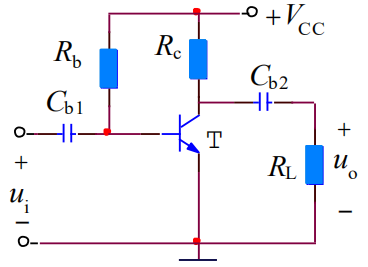
\includegraphics[scale = 0.4]{02/基本共射放大电路电路图.png}

	直流通路 : 信号源视为短路(保留内阻), 电容视为开路

	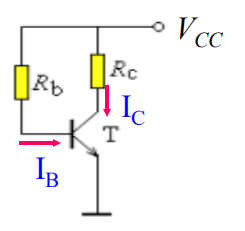
\includegraphics[scale = 0.4]{02/基本共射放大电路直流通路.png}

	交流通路 : 短路直流电压源, 电容视为短路

	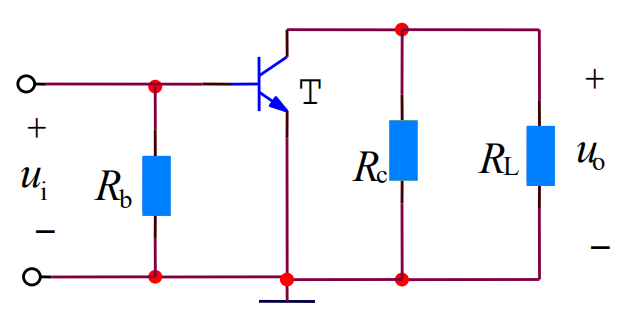
\includegraphics[scale = 0.4]{02/基本共射放大电路交流通路.png}

	估算法求静态工作点 :
	\begin{itemize}[leftmargin = 4em]
		\item 输入回路方程 : $ I_{B} = \frac{V_{CC} - U_{BE}}{R_{b}} $, $ U_{BE} $ : (锗管0.1 $ \sim $ 0.3)/(硅管0.6 $ \sim $ 0.8)
		\item 放大特性方程 : $ I_{C} = \beta I_{B} $
		\item 输出回路方程 : $ U_{CE} = V_{CC} - I_{C}R_{c} $
	\end{itemize}

	图解法求静态工作点 :
	\begin{itemize}[leftmargin = 4em]
		\item 输入回路方程 : $ I_{B} = -\frac{1}{R_{b}}U_{BE} + \frac{V_{CC}}{R_{b}} $, 与三极管的输入特性曲线的交点为静态工作点
		\item 直流负载线 : $ U_{CE} = V_{CC} - I_{C}R_{c} $, 确定两点 $ (V_{CC}, 0), (0, V_{CC} / R_{c}) $, 确定直流负载线画在三极管的输出特性曲线上
		\item 由直流负载线与 $ i_{B} = I_{BQ} $ 对应的输出特性曲线, 确定 $ I_{CQ}, U_{CEQ} $
	\end{itemize}

	图解法动态分析 :
	\begin{itemize}[leftmargin = 4em]
		\item 交流负载线 ; $ i_{C} - I_{CEQ} = -\frac{1}{R_{c} \parallel R_{L}}(u_{CE} - U_{CEQ}) $, 经过静态工作点, 比直流负载线陡
		\item 根据交流信号的变化范围, 画出工作点的变化范围
	\end{itemize}

	失真分析 :
	\begin{itemize}[leftmargin = 4em]
		\item 饱和失真 : 工作点进入饱和区, 静态工作点偏左上, NPN管输出波形削底
		\item 截止失真 : 工作点进入截止区, 静态工作点偏右下, NPN管输出波形削顶
		\item 最大不失真电压估算 : $ \min\{I_{C}(R_{c} \parallel R_{L}), U_{CEQ} - U_{CES}\} $
	\end{itemize}

	晶体三极管的小信号模型(只能求动态量, 输入信号幅度不大, $ I_{b} $流向基极的时候, 受控电流方向为集电极到发射极, 无论NPN管还是PNP管) : 

	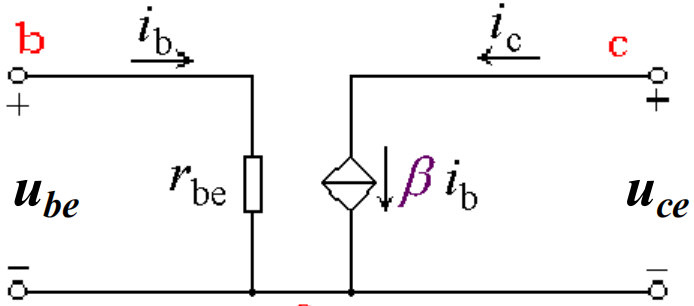
\includegraphics[scale = 0.4]{02/晶体三极管的小信号模型.png}

	其中 $ r_{be} = r_{bb'} + (1+\beta)\frac{26(mV)}{I_{E}(mA)} $

	用微变等效电路基本共射放大电路 :

	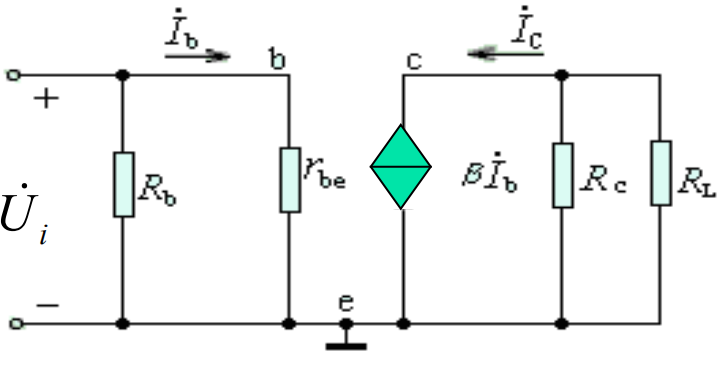
\includegraphics[scale = 0.4]{02/基本共射放大电路微变等效电路.png}

	性能指标 :
	\begin{itemize}[leftmargin = 4em]
		\item 电压增益 : $ \dot{A} = \frac{\dot{U}_{o}}{\dot{U}_{i}} = -\beta\frac{R_{c} \parallel R_{L}}{r_{be}} $
		\item 输入电阻 : $ R_{i} = \frac{\dot{U}_{i}}{\dot{I}_{i}} = R_{b} \parallel r_{be} $
		\item 输出电阻 : $ R_{o} = R_{c} $
		\item 源电压放大倍数 : $ \dot{A}_{uS} = \frac{\dot{U}_{o}}{\dot{U}_{s}} = \dot{A}_{u}\frac{R_{i}}{R_{s}+R_{i}} $, $ R_{s} $ 为信号源内阻
	\end{itemize}

	~

	\noindent
	放大电路静态工作点的稳定 :

	(1). 分压式偏置电路 :

	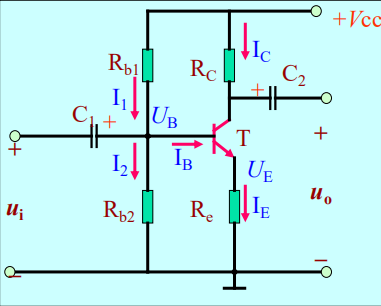
\includegraphics[scale = 0.4]{02/分压式偏置电路.png}

	$ R_{e} $ : 反馈; 稳定条件 : $ I_{2} >> I_{B}, U_{B} >> U_{BE} $

	(2). 温度补偿电路 : $ R_{b2} $ 两端并联温敏电阻

	估算分析方法 :
	\begin{itemize}[leftmargin = 4em]
		\item 直流 : $ V_{CC}-R_{b1}-R_{b2}-GND $ 路, 当作一条回路($ I_{B} $ 太小, 被忽略), $ U_{B} = \frac{R_{b2}}{R_{b1}+R_{b2}}V_{CC} $
		\item 直流 : $ I_{C} \approx I_{E} = \frac{U_{E}}{R_{e}} = \frac{U_{B} - U_{BE}}{R_{e}} \approx \frac{U_{B}}{R_{e}} $
		\item 交流 : $ \dot{A}_{u} = \frac{-\beta R_{c}}{r_{be} + (1+\beta)R_{e}}, R_{i} = R_{b1} \parallel R_{b2} \parallel [r_{be} + (1+\beta)R_{e}], R_{o} = R_{c} $
	\end{itemize}

	~

	\noindent
	基本共集放大电路 :

	电路图 :

	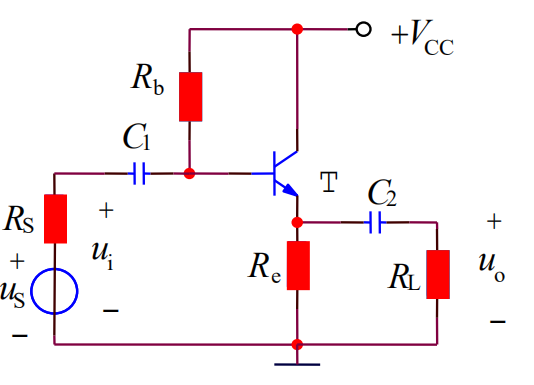
\includegraphics[scale = 0.4]{02/基本共集放大电路电路图.png}

	直流通路 :

	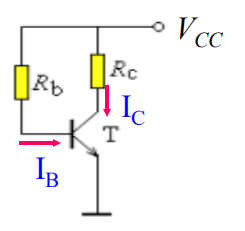
\includegraphics[scale = 0.4]{02/基本共射放大电路直流通路.png}

	微变等效电路 :

	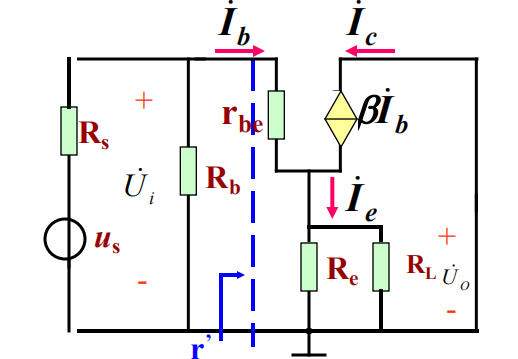
\includegraphics[scale = 0.4]{02/基本共集放大电路微变等效电路.png}

	分析 :
	\begin{itemize}[leftmargin = 4em]
		\item 直流 : $ V_{CC} = I_{B}R_{b} + U_{BE} + (1+\beta)I_{B}R_{e}, U_{CE} = V_{CC} - I_{E}R_{e} $
		\item 交流 : $ \dot{A} = \frac{(1+\beta)(R_{e} \parallel R_{b})}{r_{be} + (1+\beta)(R_{e} \parallel R_{b})}, R_{i} =  R_{b} \parallel (1+\beta)(R_{e} \parallel R_{b}), R_{o} = R_{e} \parallel \frac{r_{be} + R_{b} \parallel R_{s}}{1+\beta} $
	\end{itemize}

	特点, 应用 :
	\begin{itemize}[leftmargin = 4em]
		\item 电压增益小于但接近1, 输入输出同相
		\item 输入电阻大, 对电压信号源衰减小, 放在多级放大器输入端提高输入电阻
		\item 输出电阻小, 带负载能力强, 放在多级放大器输出端减小输出电阻
		\item 放在两级之间做缓冲
	\end{itemize}

	~

	\noindent
	基本共基放大电路 :

	电路图 :

	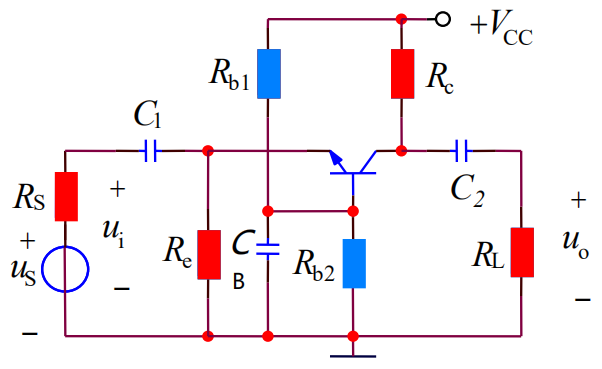
\includegraphics[scale = 0.4]{02/基本共基放大电路电路图.png}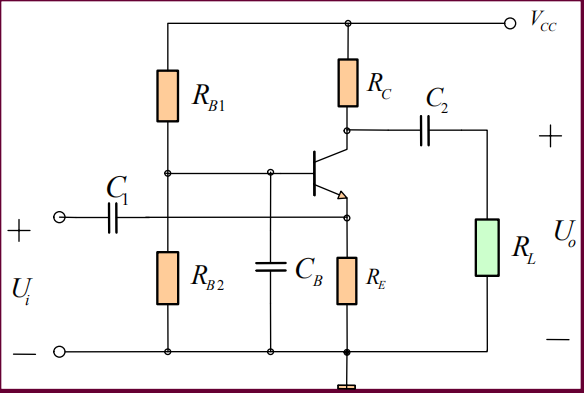
\includegraphics[scale = 0.4]{02/基本共基放大电路电路图(2).png}

	直流通路 :

	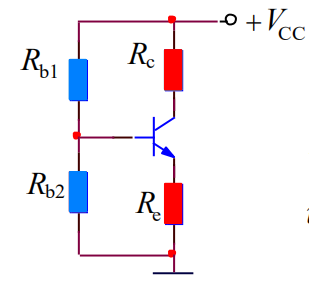
\includegraphics[scale = 0.4]{02/基本共基放大电路直流通路.png}

	微变等效电路 :

	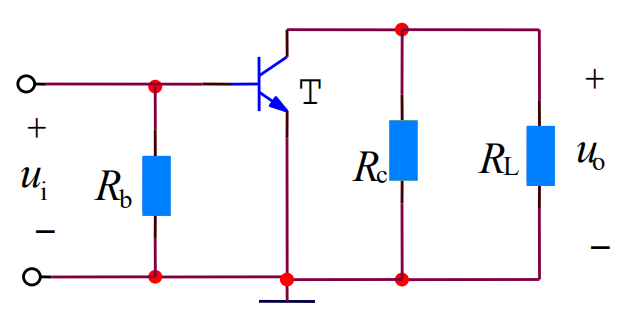
\includegraphics[scale = 0.4]{02/基本共射放大电路交流通路.png}

	分析 :
	\begin{itemize}[leftmargin = 4em]
		\item 直流 : $ U_{B} \approx \frac{R_{b2}}{R_{b1}+R_{b2}}V_{CC}, I_{C} \approx I_{E} = \frac{U_{B}-U_{BE}}{R_{e}}, U_{CE} \approx V_{CC} - I_{C}(R_{c}+R_{e}) $
		\item 交流 : $ \dot{A} = \frac{\beta(R_{c} \parallel R_{L})}{r_{be}}, R_{i} = R_{e} \parallel \frac{r_{be}}{1+\beta}, R_{o} \approx R_{c} $
	\end{itemize}

	~

	\noindent 
	场效应管的小信号模型 :

	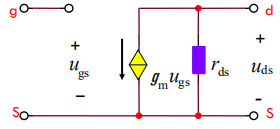
\includegraphics[]{02/场效应管小信号模型.png}

	~

	\noindent
	共源放大电路 :

	电路图 :

	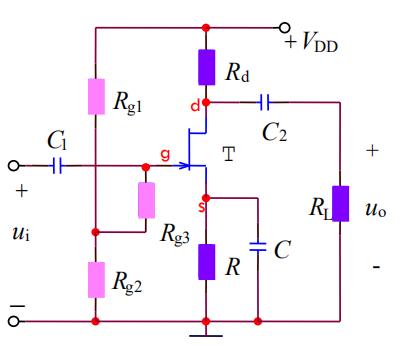
\includegraphics[scale = 0.4]{02/共源放大电路电路图.png}

	交流通路 :

	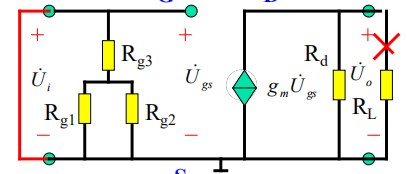
\includegraphics[scale = 0.4]{02/共源放大电路交流通路.png}

	分析 :
	\begin{itemize}[leftmargin = 4em]
		\item 直流 : $ U_{GS} = \frac{R_{g2}}{R_{g1}+R_{g2}}V_{DD} - I_{D}R, I_{D} = I_{DSS}(1-\frac{U_{GS}}{U_{P}})^{2}, U_{DS} = V_{DD} - I_{D}(R_{d}+R) $
		\item 交流 : $ \dot{A} = -g_{m}(R_{d} \parallel R_{L}), R_{i} = R_{g3} + (R_{g1} \parallel R_{g2}), R_{o} = R_{d} $
	\end{itemize}

	~

	\noindent
	共漏放大电路 :

	电路图 :

	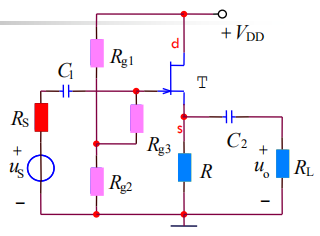
\includegraphics[scale = 0.4]{02/共漏放大电路电路图.png}

	交流通路 :

	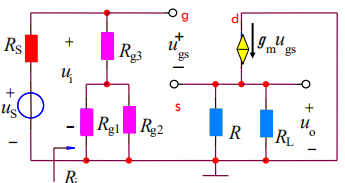
\includegraphics[scale = 0.4]{02/共漏放大电路交流通路.png}

	分析 :
	\begin{itemize}[leftmargin = 4em]
		\item 直流 : $ U_{GS} = \frac{R_{g2}}{R_{g1}+R_{g2}}V_{DD} - I_{D}R, I_{D} = I_{DSS}(1-\frac{U_{GS}}{U_{P}})^{2}, U_{DS} = V_{DD} - I_{D}R $
		\item 交流 : $ \dot{A} = \frac{g_{m}(R \parallel R_{L})}{1+g_{m}(R \parallel R_{L})} \approx 1, R_{i} = R_{g3} + (R_{g1} \parallel R_{g2}), R_{o} = R \parallel \frac{1}{g_{m}} $
	\end{itemize}

\end{document}